\documentclass[a4paper]{report}
\setlength{\headheight}{12.0pt}
\usepackage[T2A]{fontenc}
\usepackage[utf8]{inputenc}
\usepackage[russian,english]{babel}
\usepackage[left=25mm, top=20mm, right=25mm, bottom=30mm, nohead, nofoot]{geometry}
\usepackage{amsmath,amsfonts,amssymb} % математический пакет
\usepackage{fancybox,fancyhdr}
\usepackage{xcolor}
\usepackage{hyperref}
\usepackage{tkz-euclide}
\usepackage{enumitem}
\usepackage{amsmath}
\usepackage{pgfplots}
\usepackage{float}
\usepackage{fvextra}
\usepackage[cache=false]{minted}
\usepackage[figurename=Изображение]{caption}
\captionsetup[table]{name=Таблица}
\usemintedstyle{vs}

\hypersetup{colorlinks=true, allcolors=[RGB]{010 090 200}} % цвет ссылок
\newcommand{\lr}[1]{\left({#1}\right)} % команда для скобок
\pagestyle{fancy}
\fancyhf{}
\renewcommand{\headrulewidth}{0pt}
\fancyfoot[R]{\thepage}
\fancypagestyle{plain}{
    \fancyhf{}
    \fancyfoot[R]{\thepage}
    \renewcommand{\headrulewidth}{0pt}
}
\setcounter{page}{1} % счетчик нумерации страниц
\headsep=10mm
\definecolor{green_india}{HTML}{138808} % INDIA GREEN
\definecolor{green_light}{HTML}{90EE90} % LIGHT GREEN
\definecolor{green_slimy}{HTML}{299617} % SLIMY GREEN
\makeatletter
\def\@seccntformat#1{\csname #1ignore\expandafter\endcsname\csname the#1\endcsname\quad}
\let\latex@numberline\numberline
\def\numberline#1{\if\relax#1\relax\else\latex@numberline{#1}\fi}
\makeatother
\renewcommand{\thesection}{\arabic{section}.}
\renewcommand{\thesubsection}{\arabic{subsection}.}

\begin{document}
\subsection{Диаграмма пакетов}
\begin{figure}[H]
    \centering
    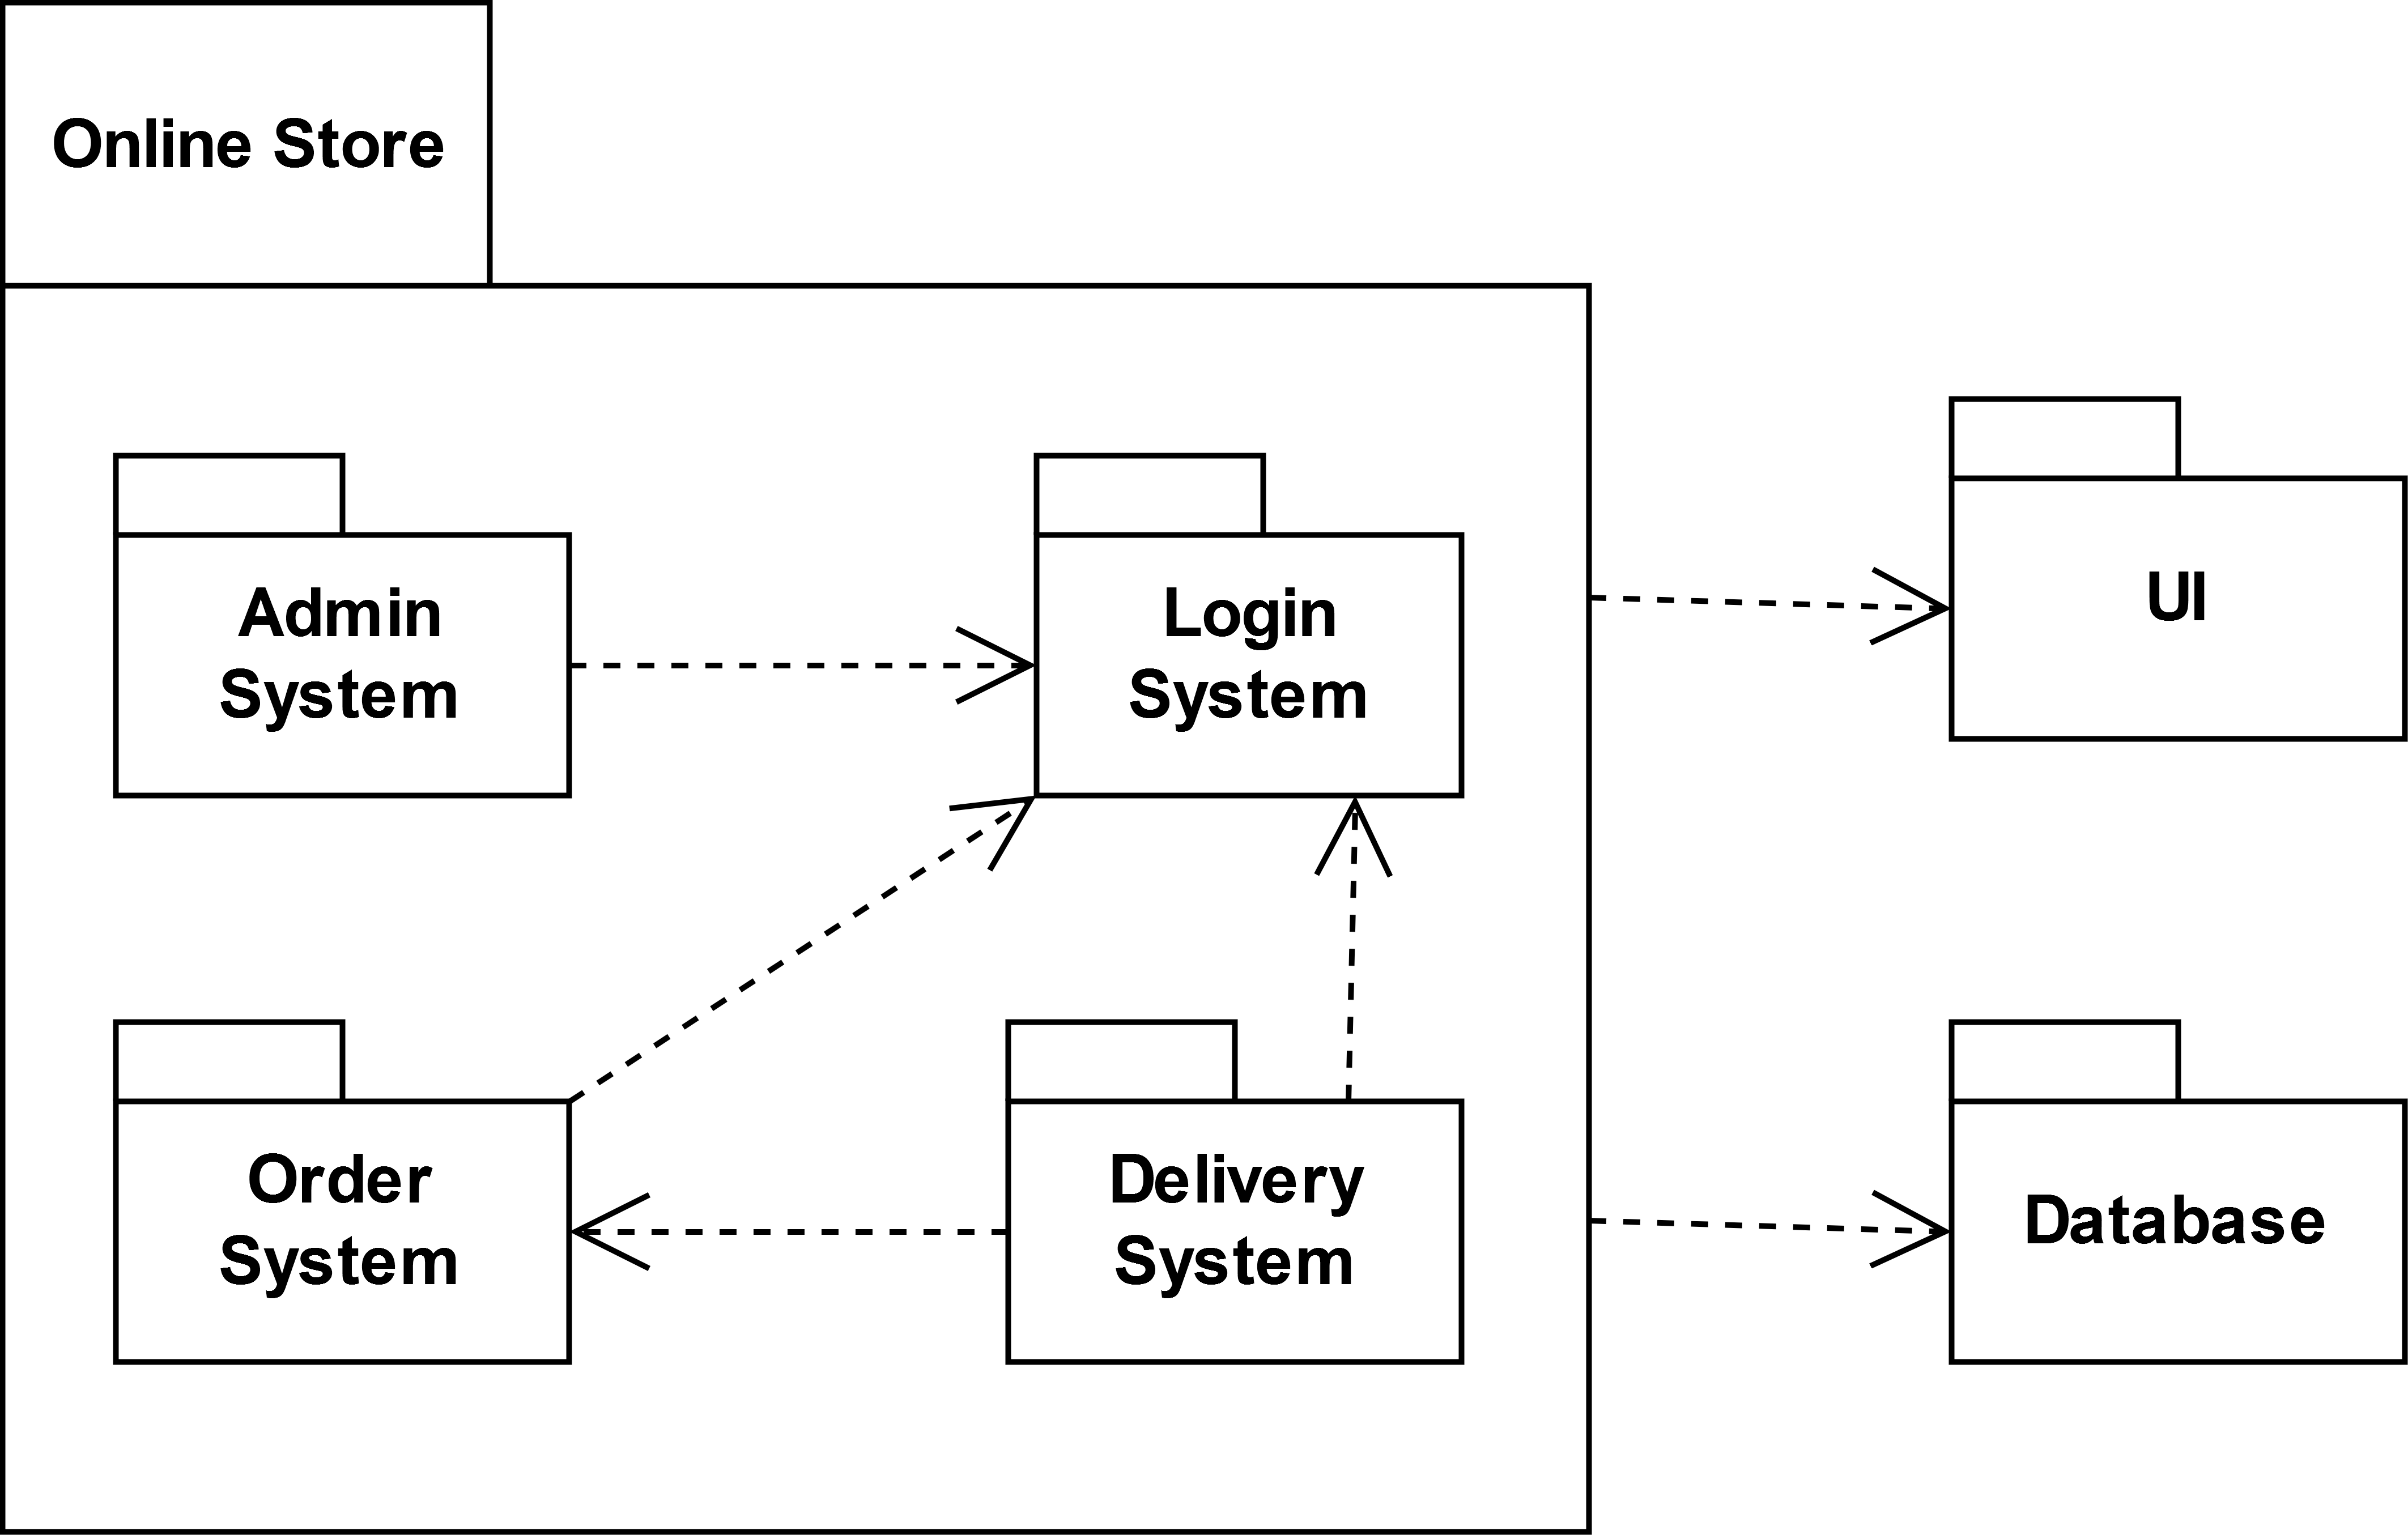
\includegraphics[width=0.6\textwidth]{Диаграмма пакетов.png}
\end{figure}
Описание:
\begin{enumerate}
    \item \textbf{Admin System:} Управляет административными функциями;
    \item \textbf{Order System:} Отвечает за обработку заказов, включая их создание, обновление и хранение;
    \item \textbf{Database:} Центральное хранилище данных, используемое всеми системами;
    \item \textbf{Online Store:} Компонент, предоставляющий функционал интернет-магазина, включая витрину товаров и работу с заказами;
    \item \textbf{Delivery System:} Система, обеспечивающая управление доставкой товаров;
    \item \textbf{Login System:} Отвечает за аутентификацию и авторизацию персонала;
    \item \textbf{UI (User Interface):} Пользовательский интерфейс для взаимодействия с системой;
    \item \textbf{Web:} Связывает пользовательский интерфейс с системой через интернет, используя соответствующую инфраструктуру.
\end{enumerate}
\subsection{Диаграмма компонентов}
\begin{figure}[H]
    \centering
    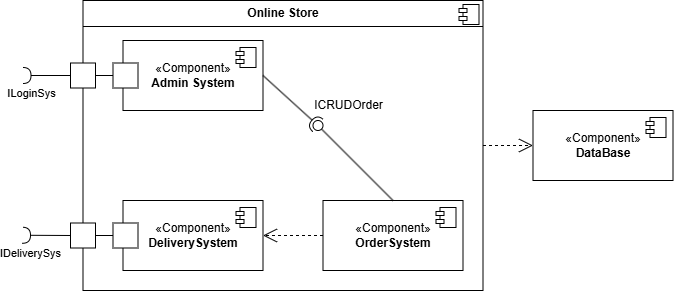
\includegraphics[width=\textwidth]{Диаграмма компонентов.png}
\end{figure}
Описание:
\begin{enumerate}
    \item \textbf{Online Store:} основной контейнер, в который входят все компоненты системы;
    \item \textbf{Admin System:} компонент, отвечающий за административные функции, такие как управление заказами и прочее. \begin{enumerate}
        \item Подключен к интерфейсу \textit{ILoginSys}, отвечает за аутентификацию пользователей;
        \item Использует интерфейс \textit{ICRUDOrder} для взаимодействия с системой управления заказами \textbf{OrderSystem}.
    \end{enumerate}
    \item \textbf{Order System:} компонент, управляющий заказами. Он обрабатывает данные заказов, которые приходят от администратора или других систем. \begin{enumerate}
        \item Связан с интерфейсом \textit{ICRUDOrder}, который предоставляет функционал для управления заказами;
        \item Также взаимодействует с \textbf{Delivery System}, передавая информацию о заказах для их доставки.
    \end{enumerate}
    \item \textbf{Delivery System:} Отвечает за обработку и управление доставкой заказов. \begin{enumerate}
        \item Подключен к интерфейсу \textit{IDeliverySys}, который может представлять внешнюю систему доставки;
        \item Получает данные о заказах из \textbf{Order System}.
    \end{enumerate}
    \item \textbf{DataBase:} Компонент базы данных, отвечающий за хранение данных системы.
\end{enumerate}
\subsection{Диаграмма развёртывания}
\begin{figure}[H]
    \centering
    \includegraphics[height=0.8\textheight]{Диаграмма развёртывания.png}
\end{figure}
Описание:
\begin{enumerate}
    \item \textbf{Web Server (веб-сервер):}\begin{enumerate}
        \item Содержит \textbf{Frontend}, предоставляющий статические ресурсы, такие как HTML, CSS и JavaScript;
        \item Этот сервер обеспечивает доступ пользователей к системе через браузер.
    \end{enumerate}
    \item \textbf{Application Server (сервер приложений):}\begin{enumerate}
        \item Хостит \textbf{Backend}, обрабатывающий бизнес-логику и API-запросы от фронтенда;
        \item Этот сервер взаимодействует с базой данных для получения или изменения данных.
    \end{enumerate}
    \item \textbf{Database Server (сервер базы данных):}\begin{enumerate}
        \item Хранит все данные системы, включая информацию о пользователях, заказах, товарах и доставках;
        \item Используется для обработки запросов на чтение и запись данных от сервера приложений.
    \end{enumerate}
\end{enumerate}
\end{document}